%%% -*- buffer-read-only: t -*-
%%% MAC=29a4abccaa0547596935b493d8a3ab60ccb9cd73
%%% LEN=9220
%%% CONTENT_SHA1=1935e7055d1888b2ac2e1220253972189c33a491
%%% 
%%% 
%%% 
%%% *** WARNING ***
%%% This is not the master copy of this file.
%%% You can edit this copy, nothing bad will happen.
%%% But it will prevent Dominique Unruh from automatically
%%% transferring changes from the master copy to this copy.
%%% Be prepared to answer to Dominique!
%%% 
%%% (If you are Dominique Unruh, disregard the above warning.)
%%% 
%%% 
%%% 
%%% 
%%% Source: /home/unruh/svn/latex/circuits/circuits.tex
%%% 
%%% 
%%% 
\documentclass[a4paper]{article}
\usepackage[T1]{fontenc}
\usepackage[ascii]{inputenc}
\usepackage[hyper]{listings}
\usepackage[most]{tcolorbox}
\usepackage{circuits}
\usepackage{geometry}

\usepackage[pdfborderstyle={/S/U/W 0.3}]{hyperref}

\makeatletter

\lstdefinestyle{example}{style=tcblatex}

\newtcblisting{example}{%
  title=Example,
  listing style=example,
  center lower}

\newenvironment{command}[2]{%
  \medskip\noindent\textbf{Command \macroanchor#1\texttt{#2}.} 
}{%
}


\newenvironment{key}[2]{%
  \medskip\noindent\textbf{Key \keyanchor{#1}\texttt{#2}.} 
}{%
}


\newcommand\nobsstring[1]{{\escapechar=-1\xdef\@tempa{\string#1}}}
\DeclareRobustCommand\macrolink[1]{\nobsstring#1\hyperref[command-\@tempa]{\texttt{\string#1}}}
\DeclareRobustCommand\macroanchor[1]{\nobsstring#1\label{command-\@tempa}\texttt{\string#1}}
\DeclareRobustCommand\keylink[1]{\hyperref[key-#1]{\texttt{#1}}}
\DeclareRobustCommand\keyanchor[1]{\label{key-#1}\texttt{#1}}
\renewcommand\sectionautorefname{Section}

\begin{document}

\title{Quantum circuits with TikZ}
\author{Dominique Unruh}
\maketitle

This is a library of macros for \href{https://sourceforge.net/projects/pgf/}{TikZ} that should facilitate the
drawing of quantum circuits.

The design goal of this library is that it should give support for
drawing circuits without interfering with the normal use of
TikZ. Thus, one can freely mix normal TikZ code and quantum circuits.

There are three basic concepts behind the macros in this library:
\begin{itemize}
\item \textbf{Wires:} A wire consists of a vertical position that
  stays the same throughout the circuit, and of a horizontal position
  that indicates upto where the wire has been drawn so far. (Or not
  drawn, in case the wire is interrupted, e.g., by a gate.) The
  horizontal position is usually updated a lot during the rendering of
  a circuit, while the vertical position stays the same unless
  explicitly changed.

  Additionally, wires can have other metadata associated with them
  (e.g., a default label).
  
  The current vertical and horizontal position of the wire can be
  accessed using \macrolink{\getWireCoord}. But in most cases, wires
  will be automatically managed by the macros in this library, in
  particular those described in \autoref{sec:wires}.
\item \textbf{Current right border:} This is the rightmost object that
  has been drawn using the library in the present circuit. (It does
  not track objects drawn directly using TikZ, use
  \macrolink{\registerRightBorderCandidate} if you want to include
  your own object in the computation of the right border.)

  The existence of the current right border allows us to easily move
  to an x position relative to the right border. (I.e., we can append
  new gates right of the last gate.)
  
  TODO: Explain how to access the current right border
\item \textbf{Current x position:} This is the default position for
  drawing, e.g., new gates. It can be updated easily using
  \macrolink\stepForward, which will move the current x position a
  given distance to the right of the current right border.

  TODO: Explain how to access the current x position
\end{itemize}

In order to initialize the circuit, you need to call
\macrolink\initializeCircuit. (Within the \verb|tikzpicture|.)

Example:

\begin{example}
\begin{tikzpicture}
  \initializeCircuit  % Initialize the circuit
  \newWire{X}{0,0}    % Create a wire at y-position 0
  \newWire{Y}{0,1}    % Create a wire at y-position 1
  \stepForward{10mm}  % Move forward by 10mm
  \node[gate={X,Y}] (U) {$U$}; % Draw a gate U at the current x position, on wires X,Y
  \stepForward{10mm}  % Move forward by 10mm
  \node[gate={X}] (H) {$H$}; % Draw a gate H at the current x position, on wires X
  \stepForward{10mm}  % Move forward by 10mm
  \drawWires{X,Y}     % Extend all wires till the end
\end{tikzpicture}
\end{example}


TODO: Document asymetric gates

\section{General}

The library is loaded using \verb|\usepackage{circuits}|.

\begin{command}\initializeCircuit{[node]}
  Initializes the circuit. Both the current x position and the current right border are initialized to
  the x-coordinate of \verb|node|. If \texttt{node} is not given, the origin is used.
\end{command}

\begin{command}\stepForward{\{distance\}}
  Sets the current x position (and the current right border) to be
  \texttt{distance} to the right of the current right border. This has
  the effect that further objects drawn by this library will be
  \texttt{distance} to the right of the circuit drawn so far.

  \texttt{distance} can be any dimension that is supported by
  TikZ. (E.g., \texttt{1pt}, \texttt{1mm}, \texttt{1}.)

  TODO: example
\end{command}

\begin{command}\registerRightBorderCandidate{\{node\}}
  Moves the current right border to the right side of the node
  \texttt{node} (unless the current right border already extends
  farther than that).

\begin{example}
\begin{tikzpicture}
  \initializeCircuit
  \newWire{X}{0,0}
  \stepForward{10mm}
  \drawWires{X}
  % Draw something (called Box) using TikZ directly
  \node (Box) at (\getWireCoord{X}) {\rule{5mm}{5mm}};
  % Make sure Box is taken into account for the current right border
  \registerRightBorderCandidate{Box}
  \stepForward{1mm} % Circuit will continue 1mm on the right of Box
  \node[gate={X}] (U) {$U$};
\end{tikzpicture}
\end{example}
\end{command}




\section{Wires}
\label{sec:wires}

TODO: describe \macrolink\newWire.

\begin{command}\getWireCoord{\{X\}}
  Expands to the name of a TikZ coordinate that marks the current
  endpoint of the wire \texttt{X}. (I.e., a coordinate with the
  current horizontal and vertical position of the wire.)

  Often, you will want to precede this with
  \macrolink{\drawWires}\texttt{\{X\}} or
  \macrolink{\skipWires}\texttt{\{X\}} to make sure the current
  endpoint of the wire matches the current x position.

\begin{example}
\begin{tikzpicture}
  \initializeCircuit
  \newWire{X}{0,0} \newWire{Y}{0,-.5}
  \stepForward{10mm}
  \drawWires{X} % Draw wire X till current x position
  % Draw an arrow pointing to wire X
  \draw[<-] (\getWireCoord{X}) -- +(0,.3) node[anchor=south] {test};
  \stepForward{10mm}
  \drawWires{X,Y}
\end{tikzpicture}
\end{example}
\end{command}

\begin{command}\labelWire{[label]\{X\}}
  Puts the label \texttt{label} (arbitrary LaTeX code) above the wire
  \texttt{X} at the current x position. If \texttt{label} is not
  given, the label last used for that wire will be reused.

  
\begin{example}
\begin{tikzpicture}
  \initializeCircuit
  \newWire{X}{0,0} \newWire{Y}{0,-.5}
  \stepForward{3mm}
  % Label wires X and Y at current x position
  \labelWire[\tiny$X$]{X}
  \labelWire[\tiny$Y$]{Y}
  \stepForward{10mm}
  % Label them again, but this time Y is labeled as Y'
  \labelWire{X}
  \labelWire[\tiny$Y'$]{Y}
  \stepForward{10mm}
  \drawWires{X,Y}
\end{tikzpicture}
\end{example}
\end{command}

\section{Gates}
\label{sec:gates}


\begin{key}{gateAsy}{=\{inputwires\}\{outputwires\}}
  A node with this key will be drawn as a gate. I.e., the node will be
  drawn large enough to cover all wires in \texttt{inputwires} and
  \texttt{outputwires}, and the \texttt{inputwires} will be drawn till
  the left border of the node, and the \texttt{outputwires} will be
  skipped till the right border of the node.

  \texttt{inputwires} and \texttt{outputwires} are comma separated
  lists of wire names.

  The current right position will be updated to the right of the gate.

  The gate will be placed with its left border at the current x
  position.

  The node must be given a name (using the TikZ-syntax
  \texttt{(name)}).

\begin{example}
\begin{tikzpicture}
  \initializeCircuit
  \newWire{X}{0,0} \newWire{Y}{0,-.5} \newWire{Z}{0,-1}
  \stepForward{3mm}
  \labelWire[\tiny$X$]{X} \labelWire[\tiny$Z$]{Z}
  \stepForward{10mm}
  % Draw a gate gateU with input wires X,Z, and with output wires X,Y
  \node[gateAsy={X,Z}{X,Y}] (gateU) {$U$};
  \stepForward{3mm}
  \labelWire[\tiny$Y$]{Y} \labelWire{X}
  \stepForward{10mm}
  % X,Y will have been skipped till the right border of gateU,
  % so we can extend them  to the end of the circuit simply using:
  \drawWires{X,Y}
\end{tikzpicture}
\end{example}
\end{key}

TODO: document


\begin{example}
\begin{tikzpicture}
  \initializeCircuit
  \newWire{X}{0,0} \newWire{Y}{0,-.5} \newWire{Z}{0,-1}
  \stepForward{3mm}
  \labelWire[\tiny$X$]{X} \labelWire[\tiny$Y$]{Y} \labelWire[\tiny$Z$]{Z}
  \stepForward{10mm}
  % Draw a Toffoli gate on X with Z,Y as controls
  \node[cnot=X,control={Z,Y}] (cnot) {};
  \stepForward{3mm}
  \stepForward{10mm}
  \drawWires{X,Y,Z}
\end{tikzpicture}
\end{example}


\section{Misc}


\begin{key}{wireInput}{=wire}
  A node with this key will be drawn as an input state for a given
  wire.  That is, it will be positioned directly on the left of the
  start of the wire.

\begin{example}
\begin{tikzpicture}
  \initializeCircuit
  \newWires{X,Y}
  \node[wireInput=X] {\small$\lvert0\rangle$};
  \node[wireInput=Y] {\small$\lvert+\rangle$};
  \stepForward{10mm}
  \labelWire[\tiny$X$]{X} \labelWire[\tiny$Y$]{Y}
  \stepForward{10mm}
  \drawWires{X,Y}
\end{tikzpicture}
\end{example}
\end{key}

\end{document}

% Local Variables:
% TeX-PDF-mode: t
% End:
